%Optics Homework_7
\documentclass[10pt,a4paper]{article}
\usepackage[UTF8]{ctex}
\usepackage{bm}
\usepackage{amsmath}
\usepackage{amssymb}
\usepackage{graphicx}
\title{光学作业\#7}
\author{陈稼霖 \and 45875852}
\date{2018.12.24}
\begin{document}
\maketitle
\section*{5-2}解:
假设物点距离透镜$s$,距离光轴$y_0$,则入射场的复振幅为
\[
\widetilde{U}_1(x,y)=A_1\exp[ik(\frac{x^2+y^2}{2s}-\frac{y_0}{s})]
\]
透镜的屏函数为
\[
\widetilde{t}_L(x,y)=t_0\exp(-ik\frac{x^2+y^2}{2F})
\]
出射场的复振幅为
\begin{align*}
\widetilde{U}_2(x,y)=&\widetilde{U}_1(x,y)\widetilde{t}_L(x,y)\\
=&A_1t_0\exp\{-ik[\frac{x^2+y^2}{2}(\frac{1}{F}-\frac{1}{s})+\frac{y_0}{s}]\}\\
=&A_1t_0\exp\{-ik[\frac{x^2+y^2}{2s'}-\frac{-\frac{s'}{s}y_0}{s'}]\}
\end{align*}
其中$s'=\frac{1}{\frac{1}{F}-\frac{1}{s'}}$。于是像点距离透镜$\frac{1}{F}-\frac{1}{s}$,距离光轴$-\frac{s'}{s}y_0$。从而横向放大率为
\[
V=\frac{-\frac{s'}{s}y_0}{y_0}=-\frac{s'}{s}
\]
若物方和像方折射率不等,设物方和像方折射率为$n_1$和$n_2$,则$\widetilde{U}_1(x,y)$式中的$k$变为$n_1k$,$\widetilde{t}_L(x,y)$式中的$k$ 变为$n_2k$,$F$变为$\frac{n_2}{\frac{n-n_1}{r_1}+\frac{n_2-n}{r_2}}$,同理可得横向放大率为
\[
V=-\frac{ns'}{n's}
\]
\section*{5-5}解:
相干照明条件下,显微镜的空间截止频率由镜头口径限制的入射光线与光轴的最大夹角决定
\[
\sin u_0=f_{\max}\lambda
\]
其倒数,空间最小分辨周期即为显微镜的最小分辨距离
\[
d_{\min}=\frac{1}{f_{\max}}=\frac{\lambda}{\sin u_0}
\]
而非相干照明条件下的最小分辨距离公式为
\[
d_{\min}=0.61\frac{\lambda}{\sin u_0}
\]
两个公式相差一个常系数,相干照明条件下显微镜的最小分辨距离稍小,分辨能力稍强。
\section*{5-6}
\subsection*{(1)}解:
远场条件要求
\begin{align*}
&\frac{\rho_0^2}{z}\ll\lambda\\
\Longrightarrow&z\gg\frac{a^2}{\lambda}=0.016m
\end{align*}
接收屏与衍射屏的距离应远大于$1.6cm$,$48cm$是一个合理的数值,即接收屏放在$48cm$远处。
\subsection*{(2)}解:
夫琅禾费衍射场要求
\[
\rho\ll z
\]
$5cm$是一个合理的数值,即接收屏幕上以衍射场中心为圆心,$5cm$ 为半径的圆内可以认为是夫琅禾费衍射场。
\subsection*{(3)}解:
零级半角宽度为
\[
\Delta\theta\approx\frac{\lambda}{a}=6.33\times10^{-3}rad=21'42''
\]
\subsection*{(4)}解:
在接收屏幕上零级的线宽度为
\[
\Delta x=z\Delta\theta=6mm
\]
\section*{5-7}
\subsection*{(1)}解:
根据傍轴条件,衍射屏与接收屏距离要远大于单缝宽度和衍射场线度
\[
z\gg a=1mm, z\gg\rho=1cm
\]
于是单缝离像面应远大于$1cm$,很可能需要大于$5cm$。
\subsection*{(2)}解:
零级半角宽度为
\[
\Delta\theta\approx\frac{\lambda}{a}=4.88\times10^{-4}rad=1'42''
\]
单缝紧贴透镜后侧,则衍射屏与接收屏之间的距离就等于像距$z=s'=80cm$,接收屏上线宽度为
\[
\Delta x=2z\Delta\theta=0.78mm
\]
\subsection*{(3)}解:
零级半角宽度同上小题,$\Delta=4.88\times10^{-4}rad=1'42''$,单缝离透镜$40cm$远,则衍射屏与接收屏之间的距离为$z=s'-40cm=40cm$,它在幕上的线宽度为
\[
\Delta x'=2z\Delta\theta=0.39mm
\]
\subsection*{(4)}解:
单缝置于透镜前方,紧贴于其左侧,则情况与第(2)小题相同,零级半角宽度为$\Delta=4.88\times10^{-4}rad=1'42''$,接收屏上线宽度为$\Delta x=2z\Delta\theta=0.78mm$。
\section*{5-9}解:
一维点阵的复振幅为
\[
\widetilde{G}(x)=\Sigma_{n=0}^{N-1}\delta(x-nd,0)
\]
后焦面上的夫琅禾费衍射衍射场即为屏函数的傅里叶频谱
\begin{align*}
\widetilde{U}(x',y')=&\int_{-\infty}^{\infty}\int_{-\infty}^{+\infty}\widetilde{G}(x,y)\exp[-i2\pi(f_xx+f_yy)]dxdy\\
=&\Sigma_{n=0}^{N-1}\exp(-2n\pi if_xd)\\
=&\frac{1-\exp(-2N\pi if_xd)}{1-\exp(-2\pi if_xd)}
\end{align*}
其中$f_x=\frac{x'}{F\lambda}$,衍射场强度分布为复振幅的模方
\begin{align*}
I'(x',y')=&\widetilde{U}(x',y')\widetilde{U}^*(x',y')=\frac{1-\exp(-2N\pi if_xd)}{1-\exp(-2\pi if_xd)}\cdot\frac{1-\exp(2N\pi if_xd)}{1-\exp{2\pi if_xd}}\\
=&\frac{2-2\cos(2N\pi f_xd)}{2-2\cos(2\pi f_xd)}=\frac{\sin^2(N\pi f_xd)}{\sin^2(\pi f_xd)}=\frac{\sin^2(N\beta x')}{\sin^2(\beta x')}
\end{align*}
其中$\beta=\frac{\pi d}{F\lambda}$。
\section*{5-10}
\subsection*{(1)}解:
后焦面上$(x',y')$点对应的空间频率为
\[
(f_x,f_y)=\frac{\sin\theta_1,\sin\theta_2}{\lambda}=\frac{(x',y')}{F\lambda}
\]
$(0,0)$点对应的空间频率为
\[
(f_x,f_y)=\frac{(0,0)}{F\lambda}=(0,0)
\]
$(0,1)$点对应的空间频率为
\[
(f_x,f_y)=\frac{(0,1)}{F\lambda}=(0,0.28mm^{-1})
\]
$(1,0)$点对应的空间频率为
\[
(f_x,f_y)=\frac{(1,0)}{F\lambda}=(0.28mm^{-1},0)
\]
$(\frac{\sqrt{2}}{2},\frac{\sqrt{2}}{2})$点对应的空间频率为
\[
(f_x,f_y)=\frac{\frac{\sqrt{2}}{2},\frac{\sqrt{2}}{2}}{F\lambda}=(2.0mm^{-1},2.0mm^{-1})
\]
$(-\frac{\sqrt{2}}{2},\frac{\sqrt{2}}{2})$点对应的空间频率为
\[
(f_x,f_y)=\frac{-\frac{\sqrt{2}}{2},\frac{\sqrt{2}}{2}}{F\lambda}=(-2.0mm^{-1},2.0mm^{-1})
\]
$(0.5,2)$点对应的空间频率为
\[
(f_x,f_y)=\frac{(0.5,2)}{F\lambda}=(1.4mm^{-1},5.6mm^{-1})
\]
$(3,-5)$点对应的空间频率为
\[
(f_x,f_y)=\frac{(3,-5)}{F\lambda}=(8.3mm^{-1},-13.9mm^{-1})
\]
$(-10,-15)$点对应的空间频率为
\[
(f_x,f_y)=\frac{(-10,-15)}{F\lambda}=(-27.8mm^{-1},-41.7mm^{-1})
\]
\subsection*{(2)}解:
系统的截止频率为
\[
f_{\max}=\frac{\sin\theta_{\max}}{\lambda}\approx\frac{D-F}{2F\lambda}=42mm^{-1}
\]
\section*{5-11}
\subsection*{(1)}答:
干涉条纹的形状是一组垂直于$y$轴的等距直线。
\subsection*{(2)}解:
物光波和参考光波在$\Sigma$平面上的相位分布分别为
\begin{align*}
&\varphi_O(y)=ky\sin\theta_O+\varphi_0\\
&\varphi_R(y)=ky\sin\theta_R=-ky\sin\theta_O
\end{align*}
其中$\varphi_0$为物光波和参考光波在$\Sigma$平面物原点处的相位差。
\subsection*{(3)}证明:
物光波和参考光波的相位差为
\[
\Delta\varphi=\varphi_O(y)-\varphi_R(y)=2kt\sin\theta_O+\varphi
\]
相邻条纹间距对应的物光波和参考光波的相位差改变$2pi$
\[
\Delta\varphi(y+\Delta y)-\Delta\varphi(y)=2k\Delta y\sin\theta_O=2\pi
\]
从而解得干涉条纹的间距公式为
\[
d=\Delta y=\frac{2\pi}{2k\sin\theta_O}=\frac{\lambda}{2\sin(\theta/2)}
\]
\subsection*{(4)}解:
当夹角$\theta=1^{\circ}$时,间距为
\[
d=\frac{632.8nm}{2\sin(1^{\circ}/2)}=36.26\mu m
\]
当夹角$\theta=60^{\circ}$时,间距为
\[
d=\frac{632.8nm}{2\sin(60^{\circ}/2)}=0.6328\mu m
\]
\subsection*{(5)}解:
当夹角$\theta=60^{\circ}$时,感官层厚度远大于干涉条纹间距$8\mu m\gg d=0.6328\mu m$,用该记录干版可以构成一张体全息图。

干版的最小分辨距离为
\[
d_{\min}=\frac{1}{3000mm^{-1}}=0.33\mu m
\]
略小于干涉条纹间距$d=0.6328\mu m$,记录干版的分辨率是匹配的。
\subsection*{(6)}解:
记录时屏上的干涉场的强度分布为
\[
I(x,y)=(\widetilde{U}_O+\widetilde{U}_R)(\widetilde{U}_O+\widetilde{U}_R)^*
\]
全息图的屏函数为
\[
\widetilde{T}(x,y)=T_0+\beta(A_O^2+A_R^2+\widetilde{U}_R^*\widetilde{U}_O+\widetilde{U}_R\widetilde{U}_O^*)
\]
用照明光束照射,产生的透射场为
\[
\widetilde{U}_T=\widetilde{U}_R'\widetilde{T}(x,y)=(T_0+\beta A_O^2+\beta A_R^2)\widetilde{U}_R'+\beta(\widetilde{U}_R'\widetilde{U}_R^*\widetilde{U}_O+\widetilde{U}_R'\widetilde{U}_R\widetilde{U}_O^*)
\]
其中$\widetilde{U}_R=\widetilde{U}_R'=A_R\exp(-iky\sin\frac{\theta}{2}), \widetilde{U}_O=A_O\exp(iky\sin\frac{\theta}{2}+i\varphi)$,于是上式可化为
\[
\widetilde{U}_T=A_0\exp(-iky\sin\frac{\theta}{2})+A_{+1}\exp(iky\sin\frac{\theta}{2}+i\varphi_0)+A_{-1}\exp(-3iky\sin\frac{\theta}{2}+i\varphi_0)
\]
其中$A_0=(T_0+\beta A_O^2+\beta A_R^2)A_R, A_{\pm1}=\beta A_R^2A_O$。 故$0$级、$+1$级、$-1$级三个衍射波均为平面波,它们分别出现在全息图后与法线成角度
\begin{align*}
\theta_{+1}=&+\frac{\theta}{2}\\
\theta_0=&-\frac{\theta}{2}\\
\theta_{-1}=&-\arcsin(3\sin\frac{\theta}{2})
\end{align*}
的方向上,如图\ref{OpticsHomework_7_5-11}。
\begin{figure}[h]
\centering
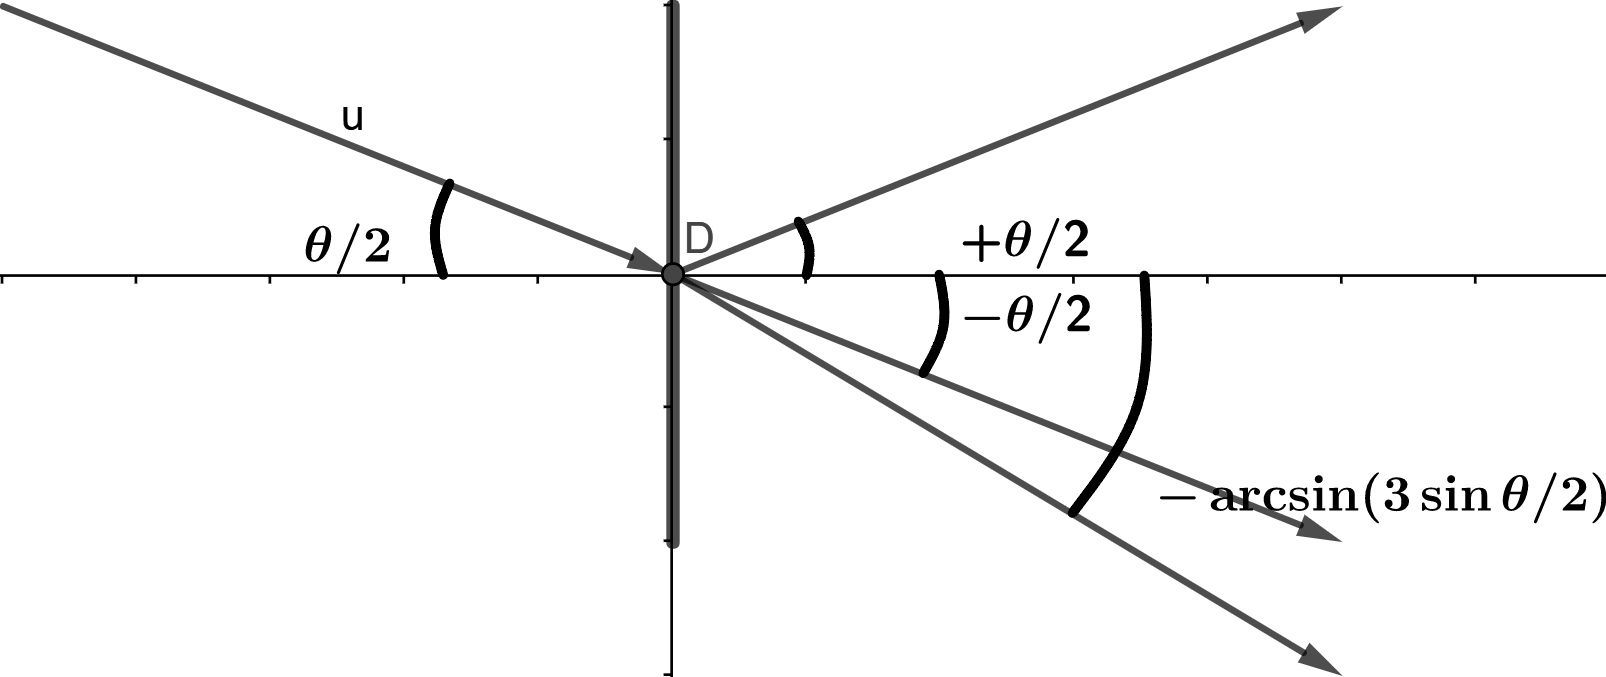
\includegraphics[scale=.2]{OpticsHomework_7_5-11.png}\\
\caption{5-11}\label{OpticsHomework_7_5-11}
\end{figure}
\section*{5-12}解:
若改用正入射的平面波再现,则照明波的复振幅变为
\[
\widetilde{U}_R'=A_R
\]
于是产生的透射场变为
\begin{align*}
\widetilde{U}_T=&\widetilde{U}_R'\widetilde{T}(x,y)=(T_0+\beta A_O^2+\beta A_R^2)\widetilde{U}_R'+\beta(\widetilde{U}_R'\widetilde{U}_R^*\widetilde{U}_O+\widetilde{U}_R'\widetilde{U}_R\widetilde{U}_O^*)\\
=&A_0+A_{+1}\exp(2iky\sin\frac{\theta}{2}+i\varphi)+A_{-1}\exp(-2iky\sin\frac{\theta}{2}-i\varphi)
\end{align*}
其中$A_0=(T_0+\beta A_O^2+\beta A_R^2)A_R, A_{+1}=A_R^2A_O, A_{-1}=A_R^2A_O$。衍射方向变为
\begin{align*}
\theta_0=&0\\
\theta_{\pm}=&\pm\arcsin(2\sin\frac{\theta}{2})
\end{align*}
\section*{5-13}
\subsection*{(1)}解:
物光波为
\[
\widetilde{U}_O=A_O\exp[ik(\frac{x^2+y^2}{2z_0}+\frac{y_0y}{z_0})]
\]
参考光波为
\[
\widetilde{U}_R=A_R
\]
记录时屏上的干涉场的强度分布为
\[
I(x,y)=(\widetilde{U}_O+\widetilde{U}_R)(\widetilde{U}_O+\widetilde{U}_R)^*
\]
全息屏的屏函数为
\[
\widetilde{T}(x,y)=T_0+\beta(A_O^2+A_R^2+\widetilde{U}_R^*\widetilde{U}_O+\widetilde{U}_R\widetilde{U}_O^*)
\]
用轴上点源$R'$发出的光照明,则照明光波为
\[
\widetilde{U}_R'=A_R'\exp(ik\frac{x^2+y^2}{2z_0})
\]
产生的透射场为
\[
\widetilde{U}_T=\widetilde{U}_R'\widetilde{T}(x,y)=(T_0+\beta A_O^2+\beta A_R^2)\widetilde{U}_R'+\beta(\widetilde{U}_R'\widetilde{U}_R^*\widetilde{U}_O+\widetilde{U}_R'\widetilde{U}_R\widetilde{U}_O^*)
\]
代入$\widetilde{U}_O, \widetilde{U}_R, \widetilde{U}_R'$得到
\[
\widetilde{U}_T=A_0\exp(ik\frac{x^2+y^2}{2z_0})+A_{+1}\exp[ik(\frac{x^2+y^2}{2\frac{z_0}{2}}+\frac{\frac{y_0}{2}y}{\frac{z_0}{2}})]+A_{-1}\exp(ik\frac{y_0y}{z_0})
\]
其中$A_0=(T_0+\beta A_O^2+\beta A_R^2)A_R', A_{+1}=\beta A_R'A_RA_O, A_{-1}=\beta A_R'A_RA_O$。因此$\pm1$级像点为位置分别为$(0,\frac{y_0}{2},\frac{z_0}{2})$和无穷远。
\subsection*{(2)}解:
若用不同的波长正入射平面波照明,则照明光波变为
\[
\widetilde{U}_R'=A_R'
\]
产生的透射场变为
\[
\widetilde{U}_T=A_0+A_{+1}\exp[ik(\frac{x^2+y^2}{2z_0}+\frac{y_0y}{z_0})]+A_{-1}\exp[ik(\frac{x^2+y^2}{2z_0}+\frac{y_0y}{z_0})]
\]
其中$A_0,A_{\pm1}$不变。因此$\pm1$级像点为位置分别为$(0,\pm y_0,z_0)$。
\end{document}
